%!TEX root = ../dokumentation.tex
\chapter{Grundlagen Laserentferungsmessung}
Um eine Entfernung zu einem Punkt mittels Licht zu bestimmen gibt es verschiedene Möglichkeiten, welche im folgenden Kapitel näher behandelt werden. Ein wichtiger Hinweiß ist zudem, dass im Zusammenhang mit dem Thema \ac{LIDAR} oftmals der Begriff "\acf{ToF}" fällt, dieser beschreibt allerdings nicht immer das direkt damit verbundene Verfahren, sondern allgemein die Entfernungsbestimmung mittels Licht. 
\section{Lichtlaufzeitmessung}
\subsection{Grundprinzip}
Das Grundprinzip der Lichtlaufzeitmessung oder auch \acf{ToF} (Abbildung: \ref{tof}), bezieht sich auf die Zeit, welche ein ausgesandter Lichtimpuls benötigt bis er wieder am Sender eintrifft.\\
\begin{figure}[H]
	\centering
	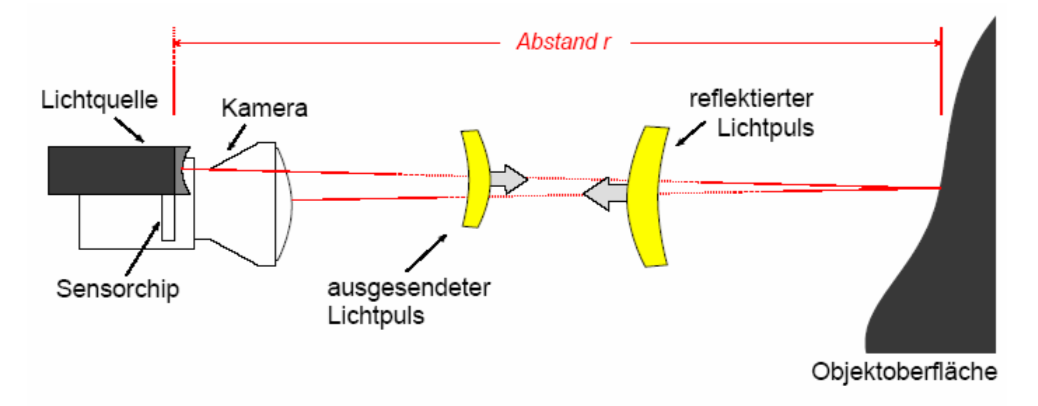
\includegraphics[width=0.75\textwidth]{images/GrundlagenLaserentfernungsmessung/ToF}
	\caption{\ac{ToF} Prinzip \cite{ToF_TUBerlin}}
	\label{tof}
\end{figure}
Dazu wird ein einzelner kurzer Lichtpult von der Lichtquelle ausgesandt, welcher dann von der Oberfläche reflektiert wird und anschließend von einem Sensorchip wieder detektiert werden kann. Über die Zeitdifferenz zwischen aussenden und detektieren des Lichtimpulses und die (doppelte) Lichtgeschwindigkeit kann anschließend auf die Entfernung des getroffenen Punktes geschlossen werden. \cite{ToF_ST}
\begin{equation}\formelentry{Berechnung der Entfernung mittels Lichtlaufzeit}
	r = \frac{t_{diff}}{2\cdot c}
\end{equation} 
\begin{flalign*}
	&r = \text{Abstand zum getroffenen Punkt } \left[m \right]&\\
	&t_{diff} = \text{Zeitdifferenz zwischen aussenden und detektieren des Lichtpulses}\left[s \right]&\\
	&c = \text{Lichtgeschwindigkeit in Luft}\left[\frac{m}{s} \right]&
\end{flalign*}
\subsection{Herrausvorderungen}
Bei dieser Technologie entstehen allerdings einige Probleme, auf welche im Folgenden eingegangen wird. 
Das erste Problem welches Auftritt ist, dass nie das gesamte ausgesandte Licht zur Detektion zur verfügung steht. Durch verschiedene Reflexionsgrade verschiedener Oberflächen und die generelle Streuung des Lichts bei auftreffen auf eine Oberfläche wir immer nur ein geringer Teil direkt zum Sensor zurückgeworfen. Daher sind hoch empfindliche Sensoren nötig um eine zuverlässige Detektion zu ermöglichen.\\
\ac{SPAD} sind für die Anwendung in einem \ac{ToF} \ac{LIDAR} System sehr gut geeignet, da eine größere Sensorfläche mit gleichbleibender Genauigkeit realisiert werden kann, und somit eine größere Streuung des reflektierten Lichts abgedeckt werden kann.\\
Ein weiteres Problem, welches \todo{Zeitmessung}

\section{Phasenverschiebung}  \label{sec:phasenverschiebung}
Das Phasenverschiebungsverfahren macht sich zu nutzen, dass bei einer ausgesandten Elektromagnetischen Welle die Phase immer größer wird bei steigender Entfernung. Durch Aussenden verschieden Frequentierter Wellen kann dann die Phasenverschiebung der Wellen bestimmt werden und daraus die Entfernung.\\
\todo{Phasenverschiebung}
\section{Triangulation}
\todo{Triangulation}